\documentclass{article}[twocolumn]
\usepackage[pdftex]{graphicx}
\usepackage[utf8]{inputenc}
\usepackage[brazil]{babel}
\usepackage{subfigure}
\usepackage{mathtools}
\usepackage{amsmath}
\usepackage{amssymb}
\usepackage{float}
\usepackage{tikz}
\usepackage[a4paper,top=2.5cm,bottom=2.5cm,left=2cm,right=2cm,marginparwidth=1.5cm]{geometry}

\title{Relat\'orio da pr\'atica 2}
\author{Kenji Yamane}

\begin{document}
	\maketitle
	\section{Parte I}
	\subsection{Quest\~ao 1}
	Query:
	\begin{verbatim}
		SELECT department_id, AVG(salary)
		FROM employees GROUP BY department_id;
	\end{verbatim}
	Print:
	\begin{figure}[H]
		\centering
		\includegraphics[width=\textwidth]{images/questao1.png}
	\end{figure}
	\newpage
	\subsection{Quest\~ao 2}
	Query:
	\begin{verbatim}
		SELECT department_id, AVG(salary)
		FROM employees GROUP BY department_id
		HAVING AVG(salary) > (SELECT AVG(salary)
		FROM employees WHERE department_id = 20);
	\end{verbatim}
	Print:
	\begin{figure}[H]
		\centering
		\includegraphics[width=\textwidth]{images/questao2.png}
	\end{figure}
	\newpage
	\subsection{Quest\~ao 3}
	Query:
	\begin{verbatim}
		SELECT employee_id, salary FROM employees
		WHERE salary < (SELECT AVG(salary) FROM employees);
	\end{verbatim}
	Print:
	\begin{figure}[H]
		\centering
		\includegraphics[width=\textwidth]{images/questao3.png}
	\end{figure}
	\newpage
	\subsection{Quest\~ao 4}
	Query:
	\begin{verbatim}
		SELECT employee_id, first_name + ' ' + last_name AS full_name
		FROM employees WHERE department_id = (SELECT department_id
		FROM employees WHERE last_name = 'Vargas');
	\end{verbatim}
	Print:
	\begin{figure}[H]
		\centering
		\includegraphics[width=\textwidth]{images/questao4.png}
	\end{figure}
	\newpage
	\subsection{Quest\~ao 5}
	Query:
	\begin{verbatim}
		SELECT employee_id, first_name + ' ' + last_name AS full_name
		FROM employees WHERE department_id IN (SELECT department_id
		FROM employees WHERE last_name IN ('Higgins', 'Lee'));
	\end{verbatim}
	Print:
	\begin{figure}[H]
		\centering
		\includegraphics[width=\textwidth]{images/questao5.png}
	\end{figure}
	\newpage
	\subsection{Quest\~ao 6}
	Query:
	\begin{verbatim}
		SELECT DISTINCT managers.employee_id, managers.first_name + managers.last_name full_name
		FROM employees workers, employees managers WHERE workers.manager_id = managers.employee_id;
	\end{verbatim}
	Print:
	\begin{figure}[H]
		\centering
		\includegraphics[width=\textwidth]{images/questao6.png}
	\end{figure}
	\newpage
	\subsection{Quest\~ao 7}
	Query:
	\begin{verbatim}
		SELECT workers.last_name "Nome Funcionario", workers.employee_id "ID Funcionario",
		managers.last_name "Nome Gerente", managers.employee_id "ID Gerente"
		FROM employees workers, employees managers WHERE workers.manager_id = managers.employee_id;
	\end{verbatim}
	Print:
	\begin{figure}[H]
		\centering
		\includegraphics[width=\textwidth]{images/questao7.png}
	\end{figure}
	\newpage
	\subsection{Quest\~ao 8}
	Query:
	\begin{verbatim}
		SELECT DISTINCT j.job_title, d.location_id FROM departments d, employees e, jobs j
		WHERE e.department_id = d.department_id AND e.job_id = j.job_id AND d.department_id = 80;
	\end{verbatim}
	Print:
	\begin{figure}[H]
		\centering
		\includegraphics[width=\textwidth]{images/questao8.png}
	\end{figure}
	\newpage
	\subsection{Quest\~ao 9}
	Query:
	\begin{verbatim}
		SELECT e.last_name, d.department_name, l.location_id, l.city
		FROM employees e, departments d, locations l
		WHERE e.department_id = d.department_id AND d.location_id = l.location_id
		AND e.commission_pct IS NOT NULL;
	\end{verbatim}
	Print:
	\begin{figure}[H]
		\centering
		\includegraphics[width=\textwidth]{images/questao9.png}
	\end{figure}
	\newpage
	\subsection{Quest\~ao 10}
	Query:
	\begin{verbatim}
		SELECT e.last_name, e.job_id, d.department_id, d.department_name
		FROM employees e, departments d, locations l
		WHERE e.department_id = d.department_id AND d.location_id = l.location_id
		AND l.city = 'Toronto';
	\end{verbatim}
	Print:
	\begin{figure}[H]
		\centering
		\includegraphics[width=\textwidth]{images/questao10.png}
	\end{figure}
	\newpage
	\subsection{Quest\~ao 11}
	Query:
	\begin{verbatim}
		SELECT e.first_name + ' ' + e.last_name full_name,
		e.job_id, d.department_name, e.salary, g.GRADE_LEVEL
		FROM employees e, departments d, grad_sal g
		WHERE e.department_id = d.department_id AND
		e.salary BETWEEN g.LOWEST_SAL AND g.HIGHEST_SAL;
	\end{verbatim}
	Print:
	\begin{figure}[H]
		\centering
		\includegraphics[width=\textwidth]{images/questao11.png}
	\end{figure}
	\newpage
	\subsection{Quest\~ao 12}
	Query:
	\begin{verbatim}
		SELECT workers.first_name + ' ' + workers.last_name "Nome Funcionario",
		       workers.hire_date "Admissao Funcionario",
		       managers.first_name + ' ' + managers.last_name "Nome Gerente",
		       managers.hire_date "Admissao Gerente"
		FROM employees workers, employees managers
		WHERE workers.manager_id = managers.employee_id
		AND workers.hire_date < managers.hire_date;
	\end{verbatim}
	Print:
	\begin{figure}[H]
		\centering
		\includegraphics[width=\textwidth]{images/questao12.png}
	\end{figure}
	\newpage
	\section{Parte II}
	\subsection{Quest\~ao 1}
	Query:
	\begin{verbatim}
		SELECT workers.first_name + ' ' + workers.last_name "Nome Funcionario",
		       workers.employee_id "ID Funcionario",
		       managers.first_name + ' ' + managers.last_name "Nome Gerente",
		       managers.employee_id "ID Gerente"
		FROM employees workers INNER JOIN employees managers
		ON workers.manager_id = managers.employee_id;
	\end{verbatim}
	Print:
	\begin{figure}[H]
		\centering
		\includegraphics[width=\textwidth]{images2/questao1.png}
	\end{figure}
	\newpage
	\subsection{Quest\~ao 2}
	Query:
	\begin{verbatim}
		SELECT e.last_name, e.job_id, d.department_id, d.department_name
		FROM employees e
		LEFT JOIN departments d ON e.department_id = d.department_id
		INNER JOIN locations l ON l.location_id = d.location_id
		WHERE l.city = 'Toronto';
	\end{verbatim}
	Print:
	\begin{figure}[H]
		\centering
		\includegraphics[width=\textwidth]{images2/questao2.png}
	\end{figure}
	\newpage
	\subsection{Quest\~ao 3}
	Query:
	\begin{verbatim}
		SELECT DISTINCT department_name FROM departments d
		LEFT JOIN employees e ON e.department_id = d.department_id
		LEFT JOIN jobs j ON e.job_id = j.job_id WHERE
		j.job_id = 'ST_CLERK';
	\end{verbatim}
	Print:
	\begin{figure}[H]
		\centering
		\includegraphics[width=\textwidth]{images2/questao3.png}
	\end{figure}
	\newpage
	\subsection{Quest\~ao 4}
	Query:
	\begin{verbatim}
		SELECT workers.last_name "Nome Funcionario", workers.employee_id "ID Funcionario",
		       managers.last_name "Nome Gerente", managers.employee_id "ID Gerente"
		FROM employees workers LEFT JOIN employees managers
		ON workers.manager_id = managers.employee_id;
	\end{verbatim}
	Print:
	\begin{figure}[H]
		\centering
		\includegraphics[width=\textwidth]{images2/questao4.png}
	\end{figure}
	\newpage
	\subsection{Quest\~ao 5}
	Query:
	\begin{verbatim}
		SELECT workers.last_name "Nome Funcionario", workers.employee_id "ID Funcionario",
		       managers.last_name "Nome Gerente", managers.employee_id "ID Gerente"
		FROM employees workers LEFT JOIN employees managers
		ON workers.manager_id = managers.employee_id WHERE workers.manager_id IS NULL;
	\end{verbatim}
	Print:
	\begin{figure}[H]
		\centering
		\includegraphics[width=\textwidth]{images2/questao5.png}
	\end{figure}
	\newpage
	\subsection{Quest\~ao 6}
	Query:
	\begin{verbatim}
		SELECT last_name "Nome Funcionario", department_id "Numero Departamento" FROM employees
		WHERE department_id = (SELECT department_id FROM
		    employees WHERE employee_id = 101);
	\end{verbatim}
	Print:
	\begin{figure}[H]
		\centering
		\includegraphics[width=\textwidth]{images2/questao6.png}
	\end{figure}
	\newpage
	\subsection{Quest\~ao 7}
	Query:
	\begin{verbatim}
		SELECT e.first_name + ' ' + e.last_name full_name, e.job_id,
		d.department_name, e.salary, gs.GRADE_LEVEL
		FROM employees e
		LEFT JOIN departments d ON e.department_id = d.department_id
		JOIN grad_sal gs ON e.salary BETWEEN gs.LOWEST_SAL AND gs.HIGHEST_SAL;
	\end{verbatim}
	Print:
	\begin{figure}[H]
		\centering
		\includegraphics[width=\textwidth]{images2/questao7.png}
	\end{figure}
	\newpage
	\subsection{Quest\~ao 8}
	Query:
	\begin{verbatim}
		SELECT workers.first_name + ' ' + workers.last_name "Nome Funcionario",
		       workers.hire_date "Admissao Funcionario",
		       managers.first_name + ' ' + managers.last_name "Nome Gerente",
		       managers.hire_date "Admissao Gerente"
		FROM employees workers
		LEFT JOIN employees managers
		ON workers.manager_id = managers.employee_id
		WHERE workers.hire_date < managers.hire_date;
	\end{verbatim}
	Print:
	\begin{figure}[H]
		\centering
		\includegraphics[width=\textwidth]{images2/questao8.png}
	\end{figure}
	\newpage
	\subsection{Quest\~ao 9}
	Query:
	\begin{verbatim}
		SELECT country_id, country_name
		FROM countries
		EXCEPT
		SELECT c.country_id, c.country_name
		FROM departments d
		LEFT JOIN locations l ON d.location_id = l.location_id
		LEFT JOIN countries c on l.country_id = c.country_id;
	\end{verbatim}
	Print:
	\begin{figure}[H]
		\centering
		\includegraphics[width=\textwidth]{images2/questao9.png}
	\end{figure}
	\newpage
	\subsection{Quest\~ao 10}
	Query:
	\begin{verbatim}
		SELECT DISTINCT j.job_id, d.department_id
		FROM jobs j
		LEFT JOIN employees e ON e.job_id = j.job_id
		LEFT JOIN departments d ON e.department_id = d.department_id
		WHERE d.department_id = 10
		UNION
		SELECT DISTINCT j.job_id, d.department_id
		FROM jobs j
		LEFT JOIN employees e ON e.job_id = j.job_id
		LEFT JOIN departments d ON e.department_id = d.department_id
		WHERE d.department_id = 20
		UNION
		SELECT DISTINCT j.job_id, d.department_id
		FROM jobs j
		LEFT JOIN employees e ON e.job_id = j.job_id
		LEFT JOIN departments d ON e.department_id = d.department_id
		WHERE d.department_id = 50;
	\end{verbatim}
	Print:
	\begin{figure}[H]
		\centering
		\includegraphics[width=\textwidth]{images2/questao10.png}
	\end{figure}
	\newpage
	\subsection{Quest\~ao 11}
	Query:
	\begin{verbatim}
		SELECT employee_id, job_id FROM job_history
		INTERSECT
		SELECT employee_id, job_id FROM employees;
	\end{verbatim}
	Print:
	\begin{figure}[H]
		\centering
		\includegraphics[width=\textwidth]{images2/questao11.png}
	\end{figure}
	\newpage
	\subsection{Quest\~ao 12}
	Query:
	\begin{verbatim}
		SELECT last_name, department_id FROM employees
		UNION
		SELECT department_name, department_id FROM departments;
	\end{verbatim}
	Print:
	\begin{figure}[H]
		\centering
		\includegraphics[width=\textwidth]{images2/questao12.png}
	\end{figure}
\end{document}
